\documentclass[11pt]{article}
\usepackage[margin=0.87in]{geometry}
\usepackage[T1]{fontenc}
\usepackage[utf8]{inputenc}
\usepackage{lmodern,microtype,booktabs,graphicx,amsmath,array,tabularx,xcolor}
\usepackage[numbers,sort&compress]{natbib}
\usepackage{hyperref}
\hypersetup{colorlinks=true,urlcolor=blue,citecolor=blue,linkcolor=blue,pdftitle={Domain-Specialized Company Memory for Grounded Marketing Recommendations},pdfauthor={Guillaume Marquis}}
\setlength{\textfloatsep}{13pt plus 2pt minus 2pt}
\setlength{\floatsep}{11pt plus 2pt minus 2pt}
\renewcommand{\topfraction}{.9}
\renewcommand{\textfraction}{.08}
\renewcommand{\floatpagefraction}{.75}
\setcounter{topnumber}{3}
\title{Domain-Specialized Company Memory for\\ Grounded Marketing Recommendations}
\author{Guillaume Marquis\thanks{AI-assisted industrial technical report. Original synthetic experiments and publicly licensed components; no customer data or human evaluation. Not peer reviewed.}}
\date{23 October 2026}
\newcommand{\ChallengeWorlds}{120}
\newcommand{\ChallengeCases}{360}
\newcommand{\ChallengeCalls}{4,320}
\newcommand{\ChallengeCompleted}{4,320}
\newcommand{\ChallengeFailures}{0}
\newcommand{\ChallengePositives}{288}
\newcommand{\ChallengeNegatives}{72}
\newcommand{\ChallengeCost}{147.68}
\newcommand{\GPTNone}{0.0}
\newcommand{\GPTCompany}{47.9}
\newcommand{\GPTGTM}{88.4}
\newcommand{\GPTFull}{100.0}
\newcommand{\GPTGain}{40.6}
\newcommand{\GPTLower}{36.7}
\newcommand{\GPTUpper}{44.4}
\newcommand{\OpusNone}{0.0}
\newcommand{\OpusCompany}{47.9}
\newcommand{\OpusGTM}{88.2}
\newcommand{\OpusFull}{98.1}
\newcommand{\OpusGain}{40.3}
\newcommand{\OpusLower}{36.3}
\newcommand{\OpusUpper}{44.3}

\begin{document}
\maketitle
\begin{abstract}
Can a marketing-specialized company memory improve next-action recommendations, or is strong generic context sufficient? We separate the policy value recoverable from retrieved evidence from the grounded feasible value actually returned by a fixed reader. A frozen benchmark contains 120 fictional company worlds, 360 multi-account cases, three compound stress levels, six executed context treatments and 4,320 actual GPT-6.1 Sol/Claude Opus 5.5 responses. On positive cases, general company context yields 47.9\% of the full-information optimum for both readers; GTM context yields 88.4\% for GPT and 88.2\% for Opus. Paired gains are 40.6 percentage points (95\% company-bootstrap interval 36.7--44.4) and 40.3 points (36.3--44.3). No company evidence yields zero grounded positive value, as expected under the evidence-required contract. The advantage is principally information selection: a generic query-word selector produces exactly the same GTM packets, and wider generic contexts close the retrieval gap. Full current context performs better, at greater API cost. On a separate one-company raw-document/wiki development set, the general wiki answers 22/22 questions correctly versus 21/22 for the marketing wiki. The results support task-aware evidence selection under a budget, not universal vertical-memory superiority, a proprietary architecture requirement or measured revenue improvement. Data, code, raw attempts, uncertainty analysis and publication figures are packaged for reproduction.

\end{abstract}
\section{Question and contribution}
Company memory should help an assistant decide what to do next, while preserving why the action is justified. The relevant engineering question is whether task-aligned context improves those decisions under an evidence budget. A larger generic company record may contain every necessary fact yet fail to present a usable chain of support to the reader.

We evaluate three visible treatments: \textbf{no company context}, \textbf{general company context}, and \textbf{GTM context}. The domain is marketing decision support. Each treatment feeds the same task, action catalog and output schema to a fixed reader, separately for GPT-6.1 Sol and Claude Opus 5.5. ``Better'' means recovering more of an explicitly defined, feasible and fully evidenced policy-priority objective. It does not mean increased revenue or expert-preferred strategy.

The contribution is an inspectable experiment and benchmark: multi-account decisions, linked prerequisites, approved policy, conflicting observations and a shared resource allowance. We measure the best decision supported by the selected context before measuring the model's returned decision. This distinguishes an information-selection bottleneck from a reader failing to use available evidence. Strong controls include a generic query-word selector, structured Markdown, native GBrain search and full current context. The query-word control is deliberately capable of falsifying the claim that a dedicated GTM architecture is necessary.

\begin{figure}[!ht]
\centering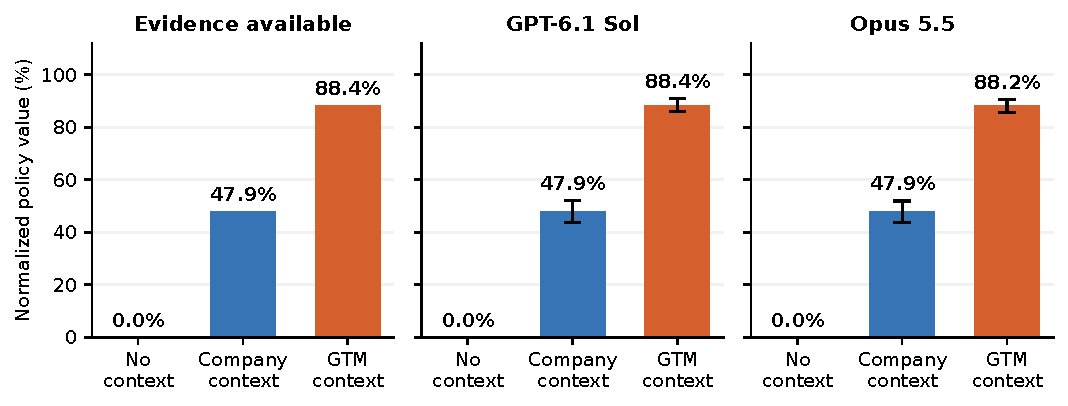
\includegraphics[width=\linewidth]{figures/challenge/headline.pdf}
\caption{The three primary context treatments. Left: the maximum policy value supported by retrieved evidence. Center/right: the grounded feasible value actually returned by each reader. Values are percentages of each positive case's full-information optimum, averaged equally by company. Reader error bars are company-clustered 95\% bootstrap intervals. No-context abstention does not earn positive decision value; negative-case safety is reported separately. Generic query-word closure produces the same GTM inputs and is an explicit control, not additional independent observations.}
\label{fig:headline}
\end{figure}

\section{Relation to prior research}
The nearest marketing work is RAMP, which already connects client-specific memory, planning and verification for audience curation~\citep{p250811120}. Its combined interventions do not isolate a memory-only effect, and our constrained account-action task is not its audience-selection benchmark. We therefore make no cross-paper numerical leaderboard claim. The retained critical review compares its methods, controls and limited human assessment with this study.

Agent-memory systems and evaluations already address persistent facts, experience, temporal updates and retrieval. Our prior review covers Hindsight, Zep, Mem0, LongMemEval and domain-specific memory evaluation~\citep{p251212818,p250113956,p250419413,p241010813,p260726072}. Wiki compilation and compression work, including WiCER and CMC, further motivates strong generic representations and fixed-reader controls~\citep{p260507068,p260932658}. Case-based reasoning and truth maintenance are older foundations for connecting evidence to actions and maintaining justified beliefs~\citep{aamodt1994,doyle1979}. Our contribution is narrower: an auditable context-budget comparison connected to feasible next-action decisions, with a control that can reproduce the specialized selector using query words alone.

Model-style agent benchmarks provide useful evaluation principles. $\tau$-bench checks domain-policy tasks against database outcomes and distinguishes average success from repeated-trial reliability \citep{taubench2024}. AppWorld allows multiple valid solutions, checks collateral changes and uses executable validation solutions; its held-out-application challenge is stronger generalization evidence than a new generator seed \citep{appworld2024}. $\tau^2$-bench composes verified subtasks and separates interaction modes to diagnose failure mechanisms \citep{tau2bench2025}. We adopt explicit constraints, acceptable alternatives and independent executable references. Our single-step, clean-record task does not reproduce their interactive environments or justify calling our scores general model capability.

\section{A controlled, more demanding task}
\subsection{Sources, decisions and stress levels}
We generate original fictional company records with eight accounts each. The three query scenarios activate four, six and eight accounts, increase corporate distractors and source conflicts, and allow respectively 16, 12 and 8~KiB of UTF-8 evidence. These are compound stress levels; their differences cannot identify the causal effect of one difficulty factor. They are counterfactual task snapshots, not longitudinal observations. Three sector labels are administrative sampling strata under the same formal schema.

Each action requires an allowed region and sector, approved policy, observed consent and signal, and a complete account $\rightarrow$ initiative $\rightarrow$ need $\rightarrow$ offering $\rightarrow$ proof chain. Proof must be approved. Some actions additionally require operational capacity, permission to share proof, or assurance evidence. Thus useful evidence can come from operations, legal or engineering, as well as marketing. Current conflicts block the affected requirement. Unapproved policy suggestions, non-response observations, future corrections and restricted notes must not become current authorized facts.

The shared catalog contains six actions with known resource costs and policy multipliers. A plan selects at most three actions for distinct accounts within one shared budget. Its value is the sum of each account's approved priority multiplied by the selected action's multiplier. These are \emph{constructed policy points}, with no calibrated relationship to commercial outcomes. Multiple plans can attain the same optimum. Readers must cite every required source, including each link and the approved priority.

The dataset is machine-authored. It has no independent human annotation or independently authored test narratives. A fresh main seed creates new worlds after development, but the relation schema, catalog and generator remain known. More worlds improve precision within this generator; they do not establish generalization to real companies or unseen task families. We separately retain the earlier exploratory raw-document/wiki evaluation on externally authored fictional company material.

\subsection{Memory treatments and shared boundaries}
All retrieval methods receive identical visible records. A common current-view layer enforces valid time, observed time, permissions and explicit same-authority supersession. Records carry entity, relation, value, authority and source identifiers. This controlled ingestion boundary removes extraction errors from the main comparison.

\begin{table}[t]
\small\centering
\begin{tabularx}{\linewidth}{lX}
\toprule
Treatment & Actual implementation and comparison boundary \\
\midrule
No company context & Shared task/catalog with no company evidence; information reference. \\
Company context & Pinned native GBrain hybrid ranking followed by domain-neutral entity/link closure, up to four link steps. \\
GTM context & The same ranking, account order and packer, with closure restricted to relations required by the shared catalog. \\
Company + query words & Generic relation filtering using words in the shared query/glossary; no GTM allowlist. Exact input equivalence is audited before aliasing any reader output. \\
Markdown control & Lossless entity-wiki representation, BM25/dense rank fusion and the same generic entity closure. \\
GBrain search & Native hybrid ranking and bounded packing alone. \\
Full current context & All permitted current records; an explicitly larger information/cost reference. \\
\bottomrule
\end{tabularx}
\caption{Controls remain visible. GBrain denotes its pinned search component with shared verified records and real embeddings, not the complete agent, graph-ingestion pipeline or hosted product. The Markdown control is an original compatible record pattern, not an official Karpathy implementation.}
\label{tab:methods}
\end{table}

The GBrain component uses PGLite and balanced hybrid search at revision \texttt{531b3b1}; query expansion and reranking are disabled. Every retrieval system uses the same real \texttt{text-embedding-3-small} vectors with 1,024 dimensions. The typed selector follows relation names and entity links, never consent truth values, priorities, eligibility labels or optimal plans. The generic query-word control receives the same task glossary. Conflicting records for a selected slot travel together. Partial slot removal cannot make a conflict disappear. A deterministic byte packer makes the input allowance auditable; actual provider tokens are also measured.

\begin{figure}[t]
\centering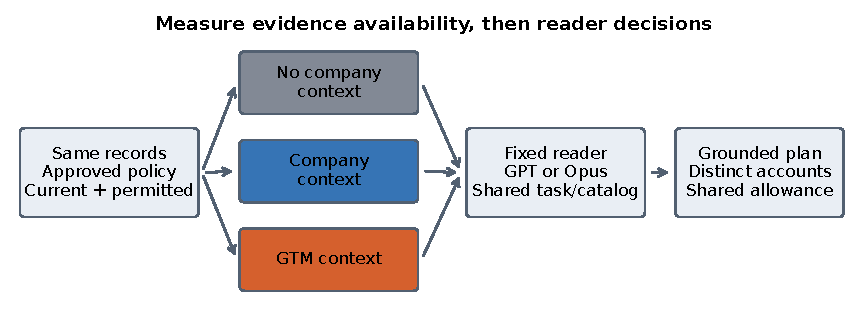
\includegraphics[width=\linewidth]{figures/challenge/design.pdf}
\caption{A common source bank and reader isolate context selection. We first compute what the selected evidence can support, then evaluate the returned plan against the full current facts and its supplied citations. The reference optimizer is a diagnostic over clean facts, not an agent baseline.}
\label{fig:design}
\end{figure}

\subsection{Readers, outcomes and uncertainty}
The new readers are \texttt{gpt-6.1-sol} with medium reasoning and \texttt{claude-opus-5-5} with adaptive thinking and high effort. Both exact model IDs and structured-output settings passed actual API checks. Each response allows up to 8,192 generated tokens; settings and prompts are constant across context treatments within a reader. Provider effort settings are not claimed compute-equivalent. There is one response per case/treatment/reader, with no automatic retries, answer repair or selection of a best attempt.

Let $V^*(q)$ be the maximum feasible policy value under full current information, $V^*_C(q)$ the maximum supported by selected context $C$, and $V_R(q)$ the value of the reader's fully grounded feasible plan. Our primary outcome is $V_R/V^*$ on cases with $V^*>0$; $V^*_C/V^*$ diagnoses evidence recoverability. An ineligible action, missing required citation, duplicate account or global budget violation invalidates the plan. Extra supplied citations are allowed, so the metric tests required-source completeness rather than citation minimality. Zero-optimum cases have a separate safety denominator. We also report exact optima, actionable coverage, abstention, failures, timing and costs. This is source-binding validation over formal records, not free-text entailment judgment or human-rated usefulness.

A development pilot covers 12 worlds and all treatments. The prospective sample rule uses the larger pilot company-level paired standard deviation across readers, targets an approximate five-percentage-point 95\% half-width, rounds to a multiple of three, and bounds the main size to 120--192 worlds. The main dataset, methods, settings and analysis are frozen before generation. The final main sample is \ChallengeWorlds{} worlds, \ChallengeCases{} cases and \ChallengeCalls{} actual reader attempts. We average positive cases within company, then weight companies equally. Confidence intervals resample companies within administrative strata, with 10,000 bootstrap replicates. The two GTM-minus-Company reader contrasts use paired random-sign tests with Holm adjustment; other contrasts are descriptive. Shared-template uncertainty is not real-market uncertainty.

An independently implemented SQLite query checks visibility and eligibility; exhaustive enumeration checks the dynamic-programming optimum. These are independent implementation checks by the same research assistant, not independent human validation. All raw responses and unsuccessful attempts remain in the artifact. Saved-output reproduction does not require paid model access; fresh inference is documented separately.

\section{Results: visible gains and their boundaries}
\subsection{The three primary treatments}
All \ChallengeCalls{} main attempts completed with saved raw responses and no technical failures. There are \ChallengePositives{} positive and \ChallengeNegatives{} zero-optimum cases. Figure~\ref{fig:headline} shows the primary contrast directly. General company context supports 47.9\% of optimal policy value; GTM context supports 88.4\%. GPT returns \GPTCompany\% versus \GPTGTM\%, and Opus returns \OpusCompany\% versus \OpusGTM\%. The paired gains are \GPTGain{} percentage points [\GPTLower, \GPTUpper] and \OpusGain{} [\OpusLower, \OpusUpper]. Both Holm-adjusted random-sign $p$-values are approximately 0.00020, at the Monte Carlo test's resolution. These intervals describe generated company worlds, not a real-company population.

GTM improves the company-mean score in 113 worlds for GPT and 112 for Opus; the remaining worlds tie. It returns a fully supported nonempty plan on 286/288 positive cases for GPT and 284/288 for Opus, versus 202/288 for Company with either reader. All six treatments safely abstain on all 72 zero-optimum cases for each reader. The no-context zero in the primary graph reflects unavailable company evidence, not zero general marketing competence.

\begin{figure}[t]
\centering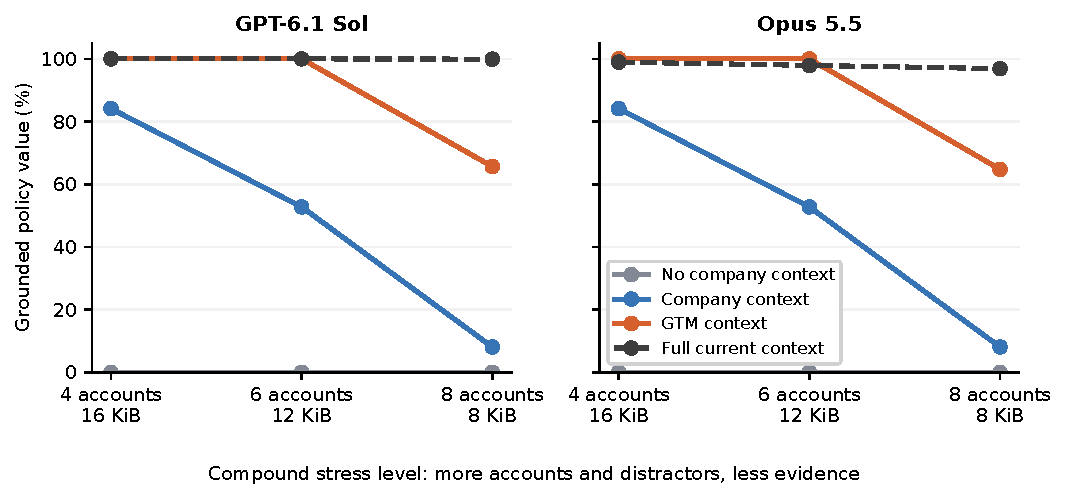
\includegraphics[width=\linewidth]{figures/challenge/difficulty.pdf}
\caption{The gap grows under the compound stress setting: Company falls from 84.1\% to 52.8\% to 8.1\%; GTM reaches 100\%, 100\% and 65.7\% (GPT) or 64.8\% (Opus). Each point contains 96 positive cases. Full current context is an information-rich reference. These settings jointly change accounts, distractions/conflicts and evidence allowance; the curves do not isolate one causal factor.}
\label{fig:difficulty}
\end{figure}

\begin{table}[t]
\centering\footnotesize\begin{tabular}{llrrrr}
\toprule
Reader & Context & Value (\%) & Exact / positive & Unsupported / all & API USD \\
\midrule
GPT-6.1 Sol & None & 0.0 & 0/288 & 0/360 & 1.06 \\
GPT-6.1 Sol & Company & 47.9 & 82/288 & 0/360 & 4.88 \\
GPT-6.1 Sol & GTM & 88.4 & 217/288 & 0/360 & 5.95 \\
GPT-6.1 Sol & Markdown & 45.7 & 73/288 & 0/360 & 4.69 \\
GPT-6.1 Sol & GBrain search & 0.0 & 0/288 & 0/360 & 5.09 \\
GPT-6.1 Sol & Full context & 100.0 & 287/288 & 0/360 & 15.62 \\
\midrule
Opus 5.5 & None & 0.0 & 0/288 & 0/360 & 4.32 \\
Opus 5.5 & Company & 47.9 & 82/288 & 0/360 & 16.06 \\
Opus 5.5 & GTM & 88.2 & 217/288 & 2/360 & 18.50 \\
Opus 5.5 & Markdown & 45.4 & 72/288 & 1/360 & 16.02 \\
Opus 5.5 & GBrain search & 0.0 & 0/288 & 0/360 & 13.40 \\
Opus 5.5 & Full context & 98.1 & 282/288 & 6/360 & 42.08 \\
\bottomrule
\end{tabular}

\caption{Every executed treatment. Value is the equal-company positive score. Exact means the full-information optimum with all required citations. Unsupported counts include any plan-contract violation; all nine observed violations are citation defects on positive cases, not ineligible actions or negative-case recommendations. USD is the observed reader subtotal for 360 calls. The identical-input query-word control adds zero calls.}
\label{tab:results}
\end{table}

\subsection{What stronger generic controls change}
The generic task-word selector produces \emph{the exact ordered evidence and messages} of GTM on 360/360 cases, verified before main generation. It uses shared query words rather than a GTM relation allowlist. Figure~\ref{fig:controls} aliases the corresponding recorded responses and explicitly does not count them as independent observations. Thus the main improvement over unconditioned entity closure does not demonstrate a need for a separate vertical database or proprietary ontology.

Structured Markdown reaches 45.7\% for GPT and 45.4\% for Opus under the main allowances. Full current context reaches \GPTFull\% and \OpusFull\%, respectively. Native GBrain search alone yields no complete eligible chain under these allowances. Its long composite query produced zero lexical matches in all 360 native executions, with real vector retrieval active. This configured search component lacks the full product's adaptive query decomposition, graph ingestion and agent loop. Its score must not be read as a whole-product capability ranking.

\begin{figure}[t]
\centering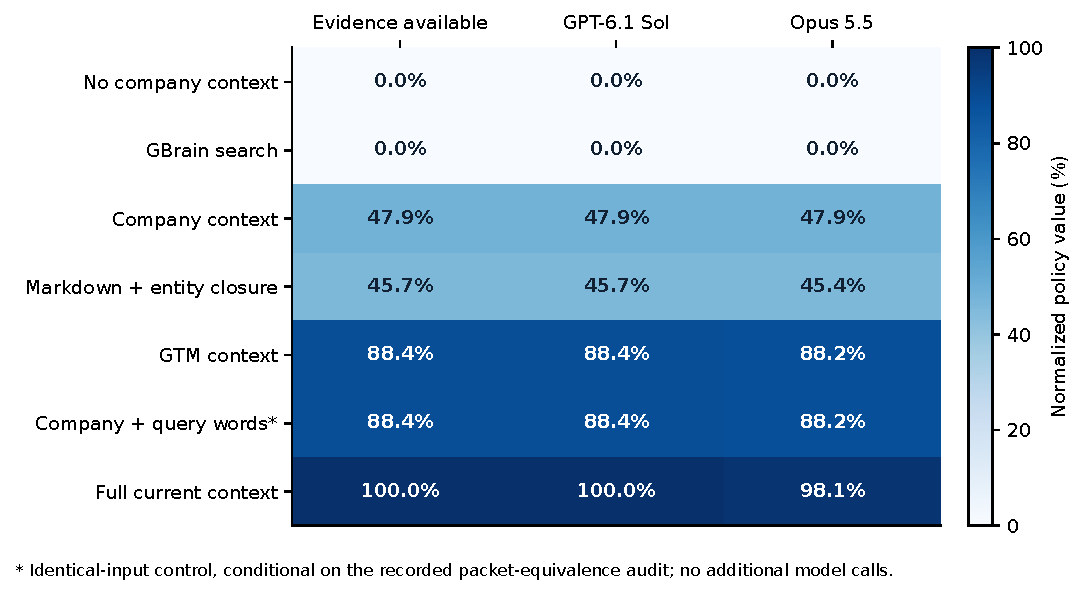
\includegraphics[width=\linewidth]{figures/challenge/controls.pdf}
\caption{All controls, including the generic method that exactly matches the specialized inputs. Evidence and reader value use the same positive denominator. The GBrain search row is a documented component configuration, not a product leaderboard. Full context has a larger input allowance.}
\label{fig:controls}
\end{figure}

The declared retrieval-only sweep further bounds the effect (Figure~\ref{fig:budget}). At 16~KiB, GTM recovers 100\% versus 59.7\% for Company. Company reaches 98.5\% at 64~KiB and 100\% at 128~KiB; every plotted method reaches 100\% at the latter allowance. These are new context computations over the same cases, with \emph{no reader calls} at the alternate budgets. Specialization improves evidence efficiency here; it does not exceed an unlimited generic information reference.

\begin{figure}[t]
\centering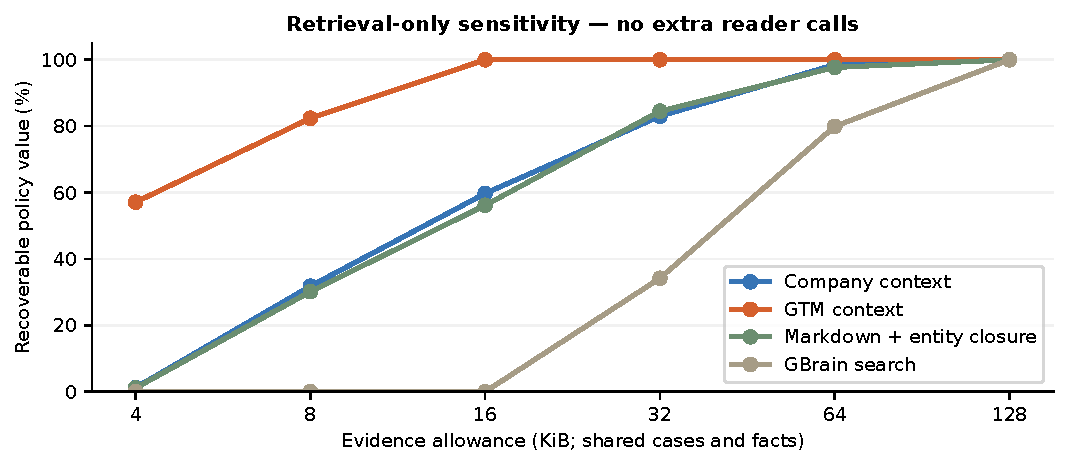
\includegraphics[width=\linewidth]{figures/challenge/budget.pdf}
\caption{Larger generic contexts close the evidence-selection gap. Each point uses all main cases and the equal-company positive aggregation; it is recoverable formal value, not measured recommendation performance at that allowance.}
\label{fig:budget}
\end{figure}

\subsection{Context quality versus reader quality}
Figure~\ref{fig:decomposition} separates missing support from unused support. Both readers attain the context-supported optimum on every Company positive case. GPT falls below its GTM context ceiling once and its full-context ceiling once. Opus has two GTM, one Markdown and six full-context citation failures; all nine plans would otherwise attain their selected context's optimum. Missing bindings concern six priorities, one capacity approval, one proof verification and one initiative-to-need link. No returned plan violates eligibility, the shared resource budget or the distinct-account rule.

A disclosed post-hoc sensitivity removes citation-binding checks while retaining context-supported eligibility and all global constraints. Opus then reaches 88.4\% with GTM and 100\% with full context; GPT scores are unchanged. The primary scores remain unchanged. This diagnosis prevents a citation defect from being misinterpreted as a bad strategic choice, while retaining the strict provenance requirement appropriate to an evidence-backed action interface.

\begin{figure}[t]
\centering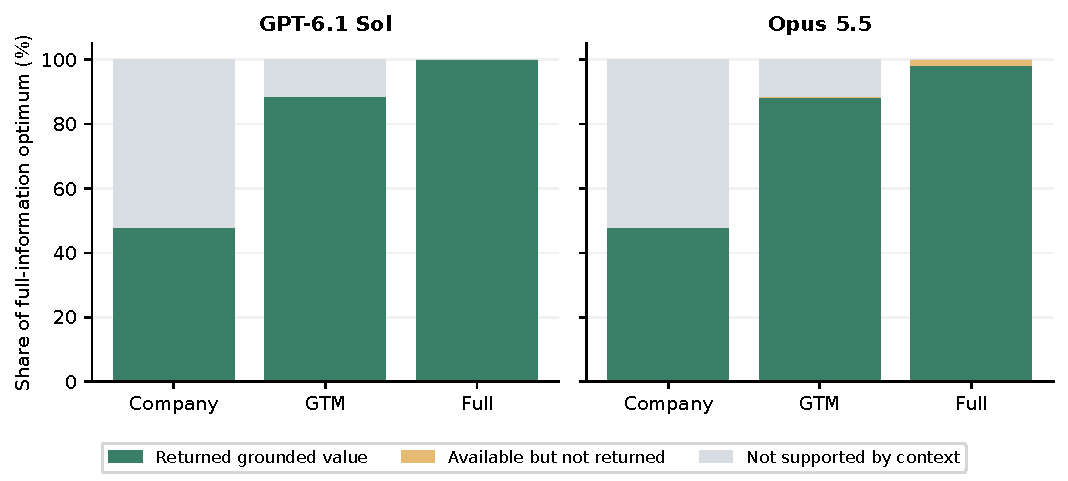
\includegraphics[width=\linewidth]{figures/challenge/decomposition.pdf}
\caption{Where value is lost. Gray is unavailable under the selected evidence; amber is available but not returned with valid citations and constraints; green is realized grounded value. This descriptive decomposition is not causal mediation analysis. Most lost value precedes the reader.}
\label{fig:decomposition}
\end{figure}

\paragraph{Qualitative trace checks.}
We inspect every reader shortfall and retain source IDs, responses and reference plans. In world 001/stress, Company supports no action, GTM only 6/66 possible points, and Markdown 48/66: the aggregate GTM advantage is not a per-case dominance guarantee. In world 000/stress, GTM preserves 30/62 points but still omits useful support. These are the first lexicographic cases of the stated retrieval-failure categories, selected descriptively after the run. In world 097/stress, Opus explicitly notices a wrong priority citation in its prose yet leaves the structured action unchanged; the validator correctly rejects that binding. GPT's world 009/stress full-context plan claims optimality at 95 points while the reference finds 105. These examples are research-assistant analysis, not blinded human judgments.

\subsection{Observed resources}
Main reader usage totals an estimated \$\ChallengeCost{}. Across availability checks, both development stages, the main, the external Opus extension and all new embedding responses, known usage totals \$183.66: 4,958 generation and 539 embedding responses, with no unknown-usage attempts in this new study. The earlier studies have separate accounting and are not included in these totals.

\begin{figure}[t]
\centering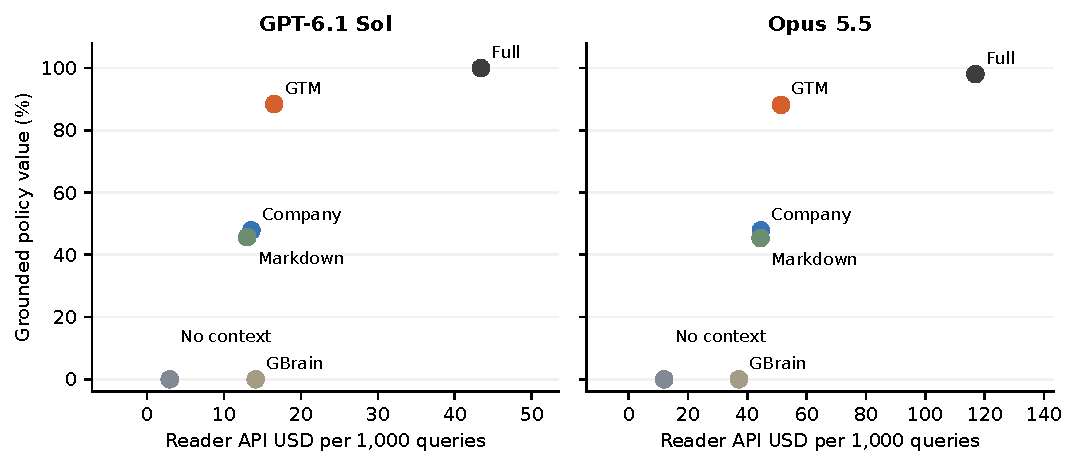
\includegraphics[width=\linewidth]{figures/challenge/cost.pdf}
\caption{Reader value versus realized API usage per 1,000 queries, including the main mix of positive and negative cases. Full context costs more and performs better. Prices, tokenizers, effort and caching differ across providers; within-reader comparisons are the intended interpretation. Ingestion, maintenance, infrastructure and practitioner time are excluded.}
\label{fig:cost}
\end{figure}

GTM slightly increases the reader bill over Company while recovering substantially more formal value. Full context costs 2.63 times GTM for GPT and 2.27 times for Opus. These are observed usage ratios, not general cost guarantees; Table~\ref{tab:resources} supplies token and elapsed-time operating points. The common clean-record boundary and shared embedding cache exclude important production costs. No savings in revenue acquisition or total ownership cost are established.

\section{External documents: an important counterexample}
\label{sec:external}
To test a different input form, we extend the earlier raw-document/wiki experiment with 132 actual Opus 5.5 calls: six contexts on 22 visible development questions from one externally authored fictional company. Its 118 source pages are MIT-licensed material from GBrain's evaluation repository. The two wikis were compiled previously by an actual query-blind GPT process, without questions or labels. We replay the exact saved contexts with Opus adaptive/high and an 8,192-token output allowance; no wiki is rewritten after seeing these answers.

\begin{figure}[t]
\centering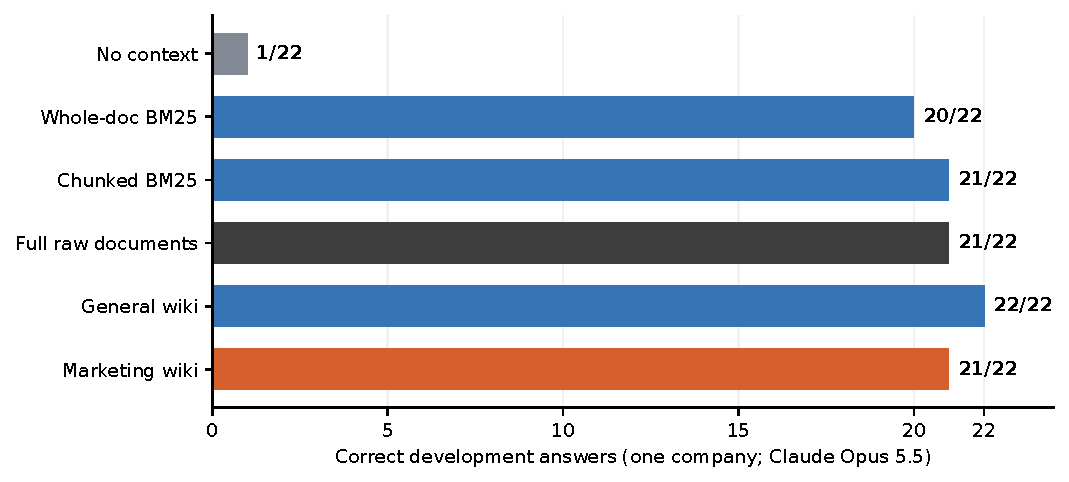
\includegraphics[width=\linewidth]{figures/challenge/external.pdf}
\caption{Exploratory raw-document/wiki QA with Opus: the general wiki outperforms the marketing wiki by one answer. This is one company with 22 development questions, not 22 independent companies or a recommendation-utility benchmark. No company-population uncertainty is inferred.}
\label{fig:external}
\end{figure}

\begin{table}[t]
\centering\small\begin{tabular}{lrrr}
\toprule
Context & Correct / 22 & Excluding ambiguous item / 21 & Reader USD \\
\midrule
No context & 1 & 1 & 0.10 \\
Whole-doc BM25 & 20 & 20 & 1.04 \\
Chunked BM25 & 21 & 21 & 1.06 \\
Full raw documents & 21 & 21 & 10.74 \\
General wiki & 22 & 21 & 2.60 \\
Marketing wiki & 21 & 20 & 2.45 \\
\bottomrule
\end{tabular}

\caption{Original upstream labels and a separately disclosed sensitivity excluding the known ambiguous July ownership question. Every original score remains retained. Reader USD excludes the earlier shared wiki compilation. Valid citation IDs do not establish semantic entailment.}
\label{tab:external}
\end{table}

The general wiki answers 22/22 correctly; the marketing wiki answers 21/22. Whole-document BM25 scores 20/22, while chunked retrieval and full raw context score 21/22. All calls complete. Excluding the known ambiguous item leaves general wiki, full raw and chunked retrieval at 21/21, but the marketing wiki at 20/21 (Table~\ref{tab:external}). This is conditional evidence against universal specialization superiority, not an estimate of a one-answer market advantage.

We review all five non-no-context errors. The marketing-wiki error misidentifies ``Dana's freight account'' in a dated handoff: the source explicitly links the phrase to Quarrendon. Both compiled wikis omit that literal phrase but retain ownership dates; Opus resolves them correctly with the general wiki and incorrectly with the marketing wiki. This is a context/reader interaction, not proof that specialization deleted the required date facts. Three raw-context errors concern the upstream July ownership ambiguity. Whole-document BM25 also misses an oversized contract clause that chunking recovers. These cases explain why compilation, packing and reference-label sensitivity need separate scrutiny. Earlier GPT/Sonnet outcomes remain archived, with different effort settings; they are not a controlled model-only comparison with this extension.

\section{What the evidence supports}
\paragraph{Context quality is an actionable engineering target.}
The controlled contrast tests whether preserving connected prerequisite evidence helps the same reader produce grounded decisions. The evidence/reader decomposition locates lost value: missing support cannot be repaired by a stronger reader without additional information. This supports measuring retrieval against downstream decision requirements, as well as relevance or answer recall. A deployment can retain a general company store while adding task-aware selection and explicit citations.

\paragraph{The generic task-word control bounds the specialization claim.}
An exact input match is a stronger mechanistic observation than a non-significant performance difference. When the generic query-word selector and GTM selector produce identical packets, their different labels do not create different information for the reader. We do not count aliased responses as additional experiments or claim an architectural moat from that comparison. Domain vocabulary and dependency-preserving packing are useful design choices; the experiment does not establish that a separate vertical database, proprietary graph or complex ontology is required.

\paragraph{Why the plots use policy value rather than abstention accuracy.}
In the earlier balanced eligibility benchmark, a model with no company evidence scored half the cases correctly by abstaining on negative examples. That number did not describe usable recommendations. The new primary graph awards value only for fully supported positive decisions and reports safety separately. It makes the information contribution visible while avoiding the interpretation that company-specific facts are a general language-model capability test.

\paragraph{Scope and unresolved evidence.}
All main histories are synthetic and follow a disclosed schema. We share a correct temporal/access boundary and verified relation fields, so ingestion quality and maintenance costs are largely outside the experiment. The compound stress levels combine several factors. Entity closure and query-word filtering are particular baseline implementations; GBrain is a search component here, not its complete autonomous product. The external wiki track remains small, developmental and from one company. There is no practitioner panel, live campaign, observed revenue, retention estimate or network-effect evidence. One response per condition does not measure repeated-run reliability. Prices are list-rate estimates from usage, not invoices or full infrastructure cost.

The product implication is to instrument evidence selection, source completeness and context cost before investing in more elaborate memory infrastructure. The release provides the data, reference solver, generic and task-conditioned selectors, actual model outputs and analysis needed to challenge that conclusion. Independent authoring, blinded practitioner review, raw-document ingestion and prospective business outcomes are the next validation steps.

\begingroup
\small
\setlength{\bibsep}{4pt}
\bibliographystyle{unsrtnat}
\bibliography{references}
\endgroup
\clearpage
\appendix
\section{Execution, provenance and reproduction}
\label{sec:reproduction}
The companion stores \texttt{main-freeze-v1.json} in \texttt{experiments/challenge/}, with methods/data revision \texttt{54ac3c01}. It records 17 code/configuration hashes, the data index and every prepared packet hash before main generation. Main seed 20261023042 creates 120 worlds and 360 cases; development seed 20261023041 creates 12 worlds and 36 cases. All 4,320 requests are reconstructed exactly, each response has a distinct provider ID, and returned model IDs match the requested frozen IDs. Source/label files remain separate; labels do not enter preparation or prompts.

The first development pilot completes 432 calls. Six unsupported decisions on two negative cases reveal timestamp-only conflict resolution. The common prompt is clarified: later dates do not supersede another supplied current record without explicit retirement. A targeted 72-call validation reuses six development cases and produces no unsupported plans. Original pilot traces, labels and source snapshots are retained; only the original pilot's paired SD (0.21244) enters the prospective sample rule. Its rounded calculation gives 72 worlds, so the declared minimum selects 120. A diagnostic field in the shared analyzer repeats the precision calculation for any analyzed run; its main-run value is not used to resize the sample.

An initial embedding receipt-path failure saves 67 actual responses before cache processing fails. Recovery loads those exact responses without reissuing them. Subsequent preparation reuses their vectors and adds 472 responses. The released vector snapshots are losslessly split into Git-sized gzip parts with per-part hashes and verification against the original compressed and uncompressed arrays. Failures, recovery notes and raw responses remain available.

GBrain is pinned at \texttt{531b3b1}; the external corpus at \texttt{6999ebc}. Fresh native execution on the first world replays three cases from released vectors with zero provider calls: native rankings and all 18 context packets match exactly. Two auxiliary Markdown full rankings differ at floating-point near-ties, while their selected packets remain identical. The frozen BM25 code iterates query terms through a Python set; saved-ranking reproduction is exact, but broader fresh-run tie stability is not claimed. The failed overly strict checker and its amended scope are retained.

Original code is MIT; specified original data/documentation are CC BY 4.0. Upstream company documents retain MIT and author credits. Proprietary services are not licensed by the companion. No production source, customer records, credentials, model weights, third-party paper PDFs or private planning history are bundled. The working repository remains private; public distribution and paper submission are separate milestones.

The companion README separates inexpensive tests, saved-output reproduction, fresh native retrieval, fresh paid inference and PDF compilation. Clean reproduction uses an extracted allowlisted package and an isolated pinned Python environment on the same host with system TeX/Pandoc/Poppler. It regenerates original datasets, reference labels, contexts, raw scores, statistics, costs and figures, verifies every file hash, and recompiles the paper and two-page investor note. It is not independent-hardware replication or fresh model inference. The final manifest and acceptance receipt identify the exact tested payload.

\section{Reader operating points and prior evidence}
\begin{table}[ht]
\centering\footnotesize\begin{tabular}{llrrrr}
\toprule
Reader & Context & Input/query & Output/query & Seconds/query & USD/1,000 \\
\midrule
GPT-6.1 Sol & None & 747 & 146 & 5.1 & 2.95 \\
GPT-6.1 Sol & Company & 4,453 & 422 & 10.2 & 13.56 \\
GPT-6.1 Sol & GTM & 4,506 & 527 & 11.2 & 16.53 \\
GPT-6.1 Sol & Full & 14,916 & 611 & 13.0 & 43.40 \\
\midrule
Opus 5.5 & None & 1,508 & 299 & 5.3 & 12.01 \\
Opus 5.5 & Company & 6,947 & 841 & 9.7 & 44.62 \\
Opus 5.5 & GTM & 6,981 & 1,174 & 12.2 & 51.39 \\
Opus 5.5 & Full & 22,214 & 1,401 & 14.4 & 116.89 \\
\bottomrule
\end{tabular}

\caption{Means across 360 main calls per treatment. Input/output are provider-reported tokens; elapsed seconds are observed response durations in the concurrent batch, not summed CPU time or service-level guarantees. USD includes recorded cache rates. Full context has a larger input footprint by design.}
\label{tab:resources}
\end{table}

Recorded base rates per million input/output tokens are \$2/\$10 for GPT and \$4/\$20 for Opus; cache accounting follows the saved provider usage categories and dated official pricing evidence. The new generation/embedding subtotal is \$183.66335244, including \$147.6757387 for main readers. These are list-price calculations, not invoices; hardware, preparation labor, maintenance and taxes are not included.

Earlier Qwen component experiments and the previous 33-world GPT/Sonnet study remain archived with their own PDFs, failures, methods and reproduction receipts. They motivated the larger sample, explicit positive-value denominator, stronger generic control and harder multi-account task. Their responses are not additional independent observations in the present analysis. The current primary and external provider experiments use Opus 5.5; Sonnet appears only in retained history.

The literature record includes bounded search queries, source dates, inclusion decisions, review depth and remaining access gaps. The new benchmark-methodology reading examines selected methods/evaluation passages of $\tau$-bench, AppWorld and $\tau^2$-bench; it is not a reproduction of their leaderboards. All 38 BibTeX records have metadata-verification receipts. Verification of citation keys and numbers does not constitute exhaustive literature coverage or peer review.

\end{document}
